% Stage: 03 ／ 説明用コード: src/ftqc
\chapter{可視化とレポート}\label{ch:visualization}

\begin{chaptergoal}
  \begin{itemize}
  \item 論理量子ビットがどの物理量子ビットに割り当てられるかを、\texttt{ftqc\_mapping\_visualizer.py} の 3 つのモデル（\texttt{mpp\_d3}／\texttt{generated\_d3}／\texttt{ls}）で読めるようになります。
  \item Stim 回路を tick（タイムスライス）ごとに展開する \texttt{stim\_timeline\_visualizer.py} の図の読み方と、\texttt{explicit}／\texttt{auto}／\texttt{instruction} の 3 つの tick ポリシーを理解します。
  \item $T$ ゲートの QPD 分岐を可視化する \texttt{t\_branch\_visualizer.py} が、$T$ を符号付きクリフォード分岐へどう展開するかを理解します。
  \item これら 3 つの基礎可視化を合成する実行レポート（\texttt{ftqc\_run\_report.py}／\texttt{ftqc\_integrated\_report.py}／\texttt{ftqc\_run\_visualizer.py}）の役割分担を理解します。
  \end{itemize}
\end{chaptergoal}

前章までで、\texttt{HybridFTQCRuntime} が論理ゲート列を受け取り、イベントへ分解し、各イベントの Stim 回路をショットごとに再生して残差を論理状態へ注入する流れを追いました。
このスタックは「論理量子ビット → 物理パッチ → Stim 回路 → tick ごとの物理操作」という複数の抽象層を貫いているため、どこかで期待とずれたとき、数値だけを眺めても原因の層を特定するのは容易ではありません。
本章では、この多層構造を層ごとに図に落とす可視化群を独立に取り上げます。
いずれも \codepath{src/ftqc/} にあり、自己完結した HTML／SVG／JSON を書き出す、依存の軽い（多くは \texttt{stim}／\texttt{qulacs} を輸入しない）モジュールです。

\begin{notebox}
  Stage: \textbf{03}。
  説明用コードは \codepath{src/ftqc/viz/ftqc_mapping_visualizer.py}、\texttt{stim\_timeline\_visualizer.py}、\texttt{t\_branch\_visualizer.py} と、それらを束ねる \texttt{ftqc\_run\_report.py}／\texttt{ftqc\_integrated\_report.py}／\texttt{ftqc\_run\_visualizer.py} を用います。
  本章の主眼は「各図を正しく読む」ことであり、巨大な HTML やログをそのまま貼るのではなく、図の構造と着眼点を示します。
\end{notebox}

\section{なぜ可視化が必要か}\label{sec:why_vis}

FTQC シミュレータのバグは、たいてい「層と層の継ぎ目」に現れます。
論理量子ビット $q$ の物理割り当てがずれていれば結果は静かに壊れますし、格子手術の seam（パッチをまたぐ縫い目）アンシラが期待どおりに配置されていなければ、\texttt{DETECTOR} が意図した対を張らず、デコードが破綻します。
$T$ ゲードを含む回路では、準確率分解（QPD）の各分岐がどこへ流れるかを追えないと、符号付き推定量の負値が「バグなのか仕様なのか」を判断できません。

本章の可視化は、3 つの基礎ツールと、それらを 1 ページに合成するレポートを提供します。ランタイム連携レポートの T 用 QEC モデルは memory のみです。

\begin{itemize}
  \item \textbf{マッピング}（\texttt{ftqc\_mapping\_visualizer.py}）：論理量子ビット $\to$ 物理量子ビット。
  \item \textbf{タイムライン}（\texttt{stim\_timeline\_visualizer.py}）：物理量子ビット $\times$ tick の実行時系列。
  \item \textbf{$T$ 分岐}（\texttt{t\_branch\_visualizer.py}）：非クリフォードの QPD 分岐ツリー。
\end{itemize}

いずれも自己完結した HTML を出力するので、実験ごとにブラウザで開いて目視確認でき、同時に機械可読な JSON manifest も残します。
これらは正解を計算する層ではなく、既に計算された構造を人間が読める形へ写す層であることに注意してください。

\section{マッピング可視化}\label{sec:mapping}

\texttt{ftqc\_mapping\_visualizer.py} は「どの物理量子ビットが各論理量子ビットを実装しているか」を描きます。
本リポジトリに存在する 3 つの割り当てモデルを 1 つの API で扱います。

\begin{itemize}
  \item \texttt{mpp\_d3}：\texttt{clifford\_ft\_full.py} が使う $d=3$ の MPP パッチ。論理量子ビット $q$ は 9 個のデータ量子ビットを持ち、物理添字は \texttt{physical = q * stride + local}（既定 \texttt{stride=9}、\texttt{local=0..8}）です。論理台は \texttt{XL=[0,3,6]}、\texttt{ZL=[0,1,2]} です。
  \item \texttt{generated\_d3}：Stim が生成した \texttt{rotated\_memory\_z} 配置を、\texttt{QUBIT\_COORDS} を解析して読み取ります（既定 \texttt{stride=40}）。\texttt{stim} は輸入せず、テキストを正規表現で解析します。
  \item \texttt{ls}：格子手術ビルダ（\texttt{CircuitLevelMerge}、\texttt{LSCnotFT}、\texttt{LSTeleportFT}）の実体を内観し、実際の座標でデータ・シンドロームアンシラ・seam アンシラを 1 つの座標系に描きます。
\end{itemize}

MPP モデルの割り当ては \texttt{build\_mpp\_assignment} が構築します。

\begin{lstlisting}[language=Python, caption={MPP パッチの割り当て構築（src/ftqc/viz/ftqc\_mapping\_visualizer.py）}]
XL = [0, 3, 6]
ZL = [0, 1, 2]
NDATA = 9

def build_mpp_assignment(n_logical, stride=NDATA, ...):
    for q in range(n_logical):
        base = q * stride
        # local=0..8 の各データに、XL/ZL の台なら役割を付ける
        # physical = base + local
        ...
\end{lstlisting}

図の読み方は次のとおりです。
各パッチは $3\times3$ の格子として描かれ、円がデータ量子ビットです。
円の色は役割を表し、$X_L$ 台は青、$Z_L$ 台は橙、両方に属する量子ビットは紫で強調されます。
円の中の数字が物理添字、下の \texttt{l0..l8} が局所添字です。
薄い矩形はスタビライザの台（$X$ 型は青、$Z$ 型は橙）を大まかな包絡として重ねたものです。

格子手術モデルでは、\texttt{build\_ls\_assignment} がビルダを内観します。
ここで重要なのは \textbf{seam アンシラ}の扱いです。

\begin{lstlisting}[language=Python, caption={seam アンシラの判定（src/ftqc/viz/ftqc\_mapping\_visualizer.py, 要約）}]
# アンシラは、その台となるデータ量子ビットの重心に置く。
# 台が 2 つ以上の物理パッチにまたがるアンシラを seam とみなす。
patches = {patch_of_index.get(s, "?") for s in support}
seam = len(patches) > 1
\end{lstlisting}

\texttt{ls} 図では、データは円・アンシラは四角で描かれ、パッチごとに色分けされます。
複数パッチにまたがる seam アンシラは赤い縁で強調されるので、「どこが 2 つのパッチを縫い合わせているか」が一目で分かります。
これは第 IV 部で見た merge の幾何が、意図どおりの縫い目を作れているかを確認する最短の手段です。

\begin{lstlisting}[language=Python, caption={プログラムからの利用（src/ftqc/viz/ftqc\_mapping\_visualizer.py の docstring より）}]
from ls_cnot_ft import LSCnotFT
from ftqc_mapping_visualizer import build_ls_assignment, write_bundle
write_bundle(build_ls_assignment(LSCnotFT(), label="LS CNOT"), "ls_cnot.html")
\end{lstlisting}

出力される JSON manifest には、パッチごとの所有物理量子ビット・$X_L/Z_L$ 台・アンシラ・seam 数（\texttt{n\_seam\_ancilla}）が含まれます。

\section{Stim タイムライン}\label{sec:timeline}

\texttt{stim\_timeline\_visualizer.py} は Stim のテキスト回路を読み、時間方向のタイムスライス（tick）に分割して、物理量子ビットごとの活動を格子状に描きます。
このモジュールも \texttt{stim} を輸入せず、\texttt{QUBIT\_COORDS}・\texttt{TICK}・クリフォードゲート・\texttt{M}/\texttt{MR}・\texttt{MPP}・ノイズ・\texttt{DETECTOR}・\texttt{OBSERVABLE\_INCLUDE}・単純な \texttt{REPEAT} ブロック（展開する）を自前で解析します。

tick の切り方は 3 つのポリシーから選べます。

\begin{itemize}
  \item \texttt{explicit}：回路中の \texttt{TICK} 命令をそのまま境界に使います。
  \item \texttt{auto}：既存の \texttt{TICK} を無視し、量子ビットが衝突しない範囲で命令を貪欲に 1 つの tick へ詰めます。\texttt{TICK} を持たない MPP レベルのトイ回路に有効です。
  \item \texttt{instruction}：活動命令を 1 つずつ別の tick に置きます。
\end{itemize}

\begin{lstlisting}[language=Python, caption={auto ポリシーの中核（src/ftqc/viz/stim\_timeline\_visualizer.py, 要約）}]
# ノイズ / DETECTOR / OBSERVABLE は直前の操作層の装飾として同じ tick に付ける。
decorative = inst.category in {"noise", "detector", "observable"}
if (not decorative) and qs and used.intersection(qs) and cur.instructions:
    ticks.append(cur)           # 量子ビットが衝突したら次の tick へ
    cur = TickSlice(tick=len(ticks)); used = set()
cur.instructions.append(inst)
if not decorative:
    used.update(qs)
\end{lstlisting}

図の読み方は次のとおりです。
横軸が tick、縦軸が物理量子ビットで、各セルはその量子ビットがその tick で行う操作を表します。
セルの色は操作の種類を示し（初期化・1 量子ビット・2 量子ビット・MPP・測定・ノイズなど）、1 つの量子ビットに複数の操作が重なる tick では、優先度の最も高い種類の色で塗り、ラベルには操作名を併記します。
2 量子ビットゲートは同じ tick 内で縦線として接続され、どの量子ビットの対に作用しているかが見えます。
格子の下には、tick ごとの測定数・検出器数のミニバーが描かれるので、シンドローム抽出のラウンド構造も俯瞰できます。

実際の出力を図\ref{fig:ch24_stim_timeline}に示します。

\begin{figure}[htbp]
  \centering
  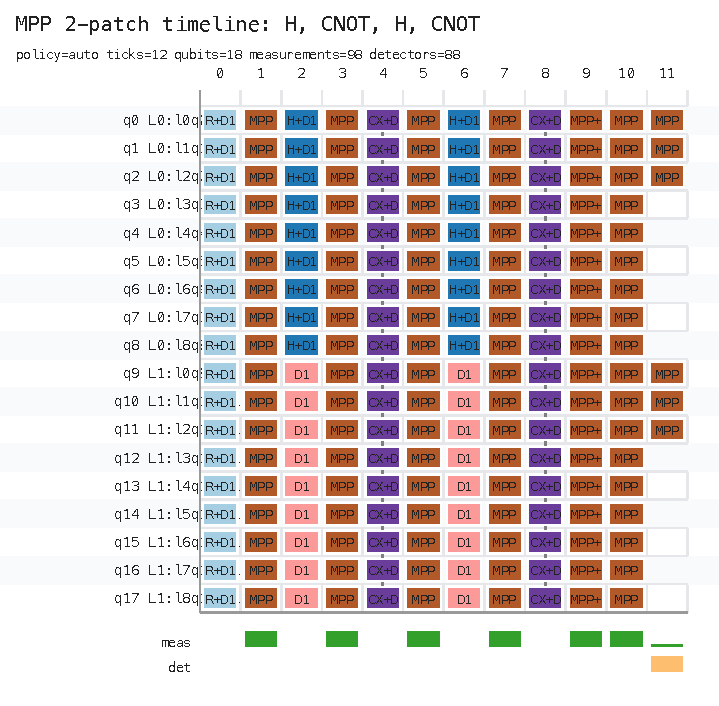
\includegraphics[width=\linewidth]{figures/ch24_stim_timeline.pdf}
  \caption{\texttt{stim\_timeline\_visualizer.py} の実出力。論理量子ビット 2 個に $H$、$\mathrm{CNOT}$、$H$、$\mathrm{CNOT}$ を順に適用した MPP 回路を \texttt{tick\_policy="auto"}・\texttt{stride=9} で可視化しています（tick 数 12、物理量子ビット 18 個、測定 98 回、検出器 88 個）。行ラベルは \texttt{q0 L0:l0} のように論理パッチ \texttt{L} と局所番号 \texttt{l} に分解されています。$H$ は $L0$ の 9 量子ビット全体にかかる transversal H（青）、$\mathrm{CNOT}$ は 2 パッチ間の transversal CX（紫）で、対応する量子ビットが縦線で結ばれます。褐色は MPP によるスタビライザ測定ラウンドです。}
  \label{fig:ch24_stim_timeline}
\end{figure}

\texttt{stride} を渡すと、行ラベルが \texttt{q7 L0:l7} のように「論理 \texttt{L}・局所 \texttt{l}」へ分解され、論理パッチごとのまとまりが読めます。
このとき manifest には、tick ごとに活動している論理パッチ数の分布（\texttt{patch\_concurrency\_counts}）も入ります。

\begin{warningbox}
  \texttt{explicit} ポリシーを \texttt{TICK} の無い回路に適用すると、全命令が 1 つの巨大な tick に潰れてしまいます。
  このモジュールはその状況を検出し、HTML に「\texttt{--tick-policy auto} を使うと量子ビット衝突を避けて自動でタイムスライス化できる」旨の警告を出します。
  MPP レベルのトイ回路では \texttt{auto} を既定にするのが安全です。
\end{warningbox}

\section{T 分岐可視化}\label{sec:t_branch}

\texttt{t\_branch\_visualizer.py} は、非クリフォードの $T$／$T^\dagger$ をゲートカット（QPD）で符号付きクリフォード分岐に展開する様子を描きます。
$T$ の分解は次の 3 項です。

\[
T = \tfrac12 I + \tfrac{1}{\sqrt2}\,S - \tfrac{\sqrt2-1}{2}\,Z,
\qquad
T^\dagger = \tfrac12 I + \tfrac{1}{\sqrt2}\,S^\dagger - \tfrac{\sqrt2-1}{2}\,Z.
\]

\begin{lstlisting}[language=Python, caption={T の QPD 項（src/ftqc/viz/t\_branch\_visualizer.py）}]
SQRT2 = math.sqrt(2.0)
T_QPD_TERMS = (
    ("I", 0.5),
    ("S", 1.0 / SQRT2),
    ("Z", -(SQRT2 - 1.0) / 2.0),
)
\end{lstlisting}

係数の絶対値の和がその $T$ の $\gamma$ で、$\gamma = \tfrac12 + \tfrac{1}{\sqrt2} + \tfrac{\sqrt2-1}{2} = \sqrt2$ です。
$T$ が $k$ 個あれば分岐は $3^k$ 本、全体の $\gamma$ は $(\sqrt2)^k$、モンテカルロ推定の分散オーバーヘッドは $\gamma^2$ になります。
図の読み方の要点は、分岐の\textbf{行き先}です。

\begin{itemize}
  \item \textbf{$I$／$Z$ 分岐}はクリフォードのみなので、通常の Stim／クリフォード QEC チャンクへ流せます。
  \item \textbf{$S$／$S^\dagger$ 分岐}は位相ゲートなので、\texttt{LS-S} シェル（第 IV 部）へルーティングされます。図では黄色でマークされ、各分岐に \texttt{...\_ls\_s\_shell} というシェルラベルが付きます。
\end{itemize}

分岐ツリーの SVG は、$T$ の数だけ深さが増え、各ノードにその接頭辞までの累積係数が表示されます。
負係数（$Z$ 項）を通った分岐は赤系の色で描かれ、これが後処理の符号付き推定量で負の重みを持つことを示します。
分岐数が既定の上限（\texttt{max\_branches=243}、すなわち $3^5$）を超えると、ツリーは省略され「JSON／表を見よ」という案内に切り替わります。これが「巨大ログを載せすぎない」ための実装上の歯止めです。

このモジュールは小さな NumPy 状態ベクトルで理想分布も計算し、QPD 再構成分布・有限ショットの符号付き推定量・理想 $T$ 分布を並べて表示します。
符号付き推定量に小さな負値が出ることがあるのは仕様であり（$Z$ 分岐の負係数を後処理で復元するため）、バグではない——この判断を図が支えます。

\section{実行レポート}\label{sec:reports}

前 3 節のツールは層ごとの単体ビューでした。
残る 3 モジュールは、それらを\textbf{同一の run／操作}について 1 ページに合成します。

\subsection{ftqc\_integrated\_report.py}

\texttt{ftqc\_integrated\_report.py} は、1 つの格子手術操作を 3 つの視点で縦に積みます。
(1) アーキテクチャ／依存グラフ、(2) 論理 $\to$ 物理マッピング、(3) 実行時系列（tick）です。
依存グラフは第18章の 7 ファイル図（\texttt{fig:deps}）に対応し、選んだ操作が使うファイルを橙色で強調します。

\begin{lstlisting}[language=Python, caption={操作ごとの強調ファイル（src/ftqc/viz/ftqc\_integrated\_report.py）}]
_OP_HIGHLIGHT = {
    "merge_zz": {"sh", "cm", "gm"},
    "cnot":     {"sh", "cn", "gm"},
    "t":        {"sh", "cn", "tg", "gm"},
    ...
}
\end{lstlisting}

3 つの視点は同じビルダ実体から生成されるので、「同じ回路を 3 つの角度から見ている」ことが保証されます。

\subsection{ftqc\_run\_visualizer.py}

\texttt{ftqc\_run\_visualizer.py} は、現行 runtime の \texttt{plan(gates)} を可視化へ配線する\textbf{非侵襲}なブリッジです。
\texttt{HybridFTQCRuntime} は各イベントの Stim 回路を内部で構築して即サンプル・デコードし、回路自体を \texttt{QECReport} に保持しません。
そこでこのブリッジは、plan の各イベントに対して可視化用の代表回路を構築し、タイムラインへ渡します。LS-CNOT イベントには LS-CNOT ビルダを使います。空の Clifford chunk と単独の S/T イベントは汎用の memory 回路で表します。これらは statevector 経路の内部回路や、QPD の全分岐を記録した実行トレースではありません。

\begin{lstlisting}[language=Python, caption={plan のイベントを回路へ再構築（src/ftqc/viz/ftqc\_run\_visualizer.py, 要約）}]
for ev in runtime.plan(gates):
    if isinstance(ev, CliffordChunk):
        circ = _clifford_circuit(ev.gates, n, p, tail)
    elif isinstance(ev, LSCnotEvent):
        circ = build_ls_cnot_shell(p=p, noise=True).circuit
        ls_builder = LSCnotFT()          # マッピング図用のビルダ実体
    elif isinstance(ev, SpecialGate):
        circ = _clifford_circuit([], n, p, tail)  # 汎用 memory 回路による代表表示
\end{lstlisting}

こうして「論理ゲート列 $\to$ イベントごとの代表回路 $\to$ tick」を一望できます。これは runtime が実際に実行した全回路の記録ではありません。
$T$ を含む場合は、同じゲート列を \texttt{t\_branch\_visualizer} にも渡して QPD の分岐構造を別に表示します。QPD モードでは $I/Z$ 分岐が memory 経路、$S/S^\dagger$ 分岐が LS-S に対応しますが、run レポートは全分岐の実行トレースではありません。

\subsection{ftqc\_run\_report.py}

\texttt{ftqc\_run\_report.py} は、1 つの run を \textbf{4 視点}で 1 ページに束ねるレポートです。T 用 QEC モデルとして実装されているのは memory のみです。
(1) 依存グラフ（全イベントが使うファイルの和集合を強調）、(2) ベースの論理 $\to$ 物理（\texttt{mpp\_d3} データパッチ）、(3) イベント別の（LS ならマッピング $+$）tick、(4) $T$ を含むなら QPD 分岐です。
3 つの可視化と 2 つのブリッジをライブラリとして合成します。依存図、イベント一覧、QPD 図は同じ入力ゲート列と plan を基にしますが、タイムラインは上記の代表回路を示します。

\begin{lstlisting}[language=Python, caption={4 視点レポートの合成（src/ftqc/viz/ftqc\_run\_report.py, 要約）}]
rt = HybridFTQCRuntime(n_logical, p_phys=p_phys, cnot_mode=cnot_mode,
                       nonclifford_mode=nonclifford_mode)
evs = event_circuits(rt, gates)                 # 同じ plan を共有
highlight = set().union(*[e["highlight"] for e in evs])
dep_svg   = build_dependency_svg(highlight)     # (1) 依存グラフ
base_map  = fmv.build_mpp_assignment(n_logical, ...)   # (2) ベース割り当て
# (3) 各イベントの代表回路のタイムライン、(4) T の QPD 分岐図
\end{lstlisting}

読むときは上から下へ、抽象（どのファイル・どの論理割り当て）から具体（tick ごとの物理操作・分岐）へ降りていくのが定石です。

\section{やること・スコープ外}\label{ch24:scope}

\subsection{やること}

\begin{itemize}
  \item 3 つの割り当てモデル（\texttt{mpp\_d3}／\texttt{generated\_d3}／\texttt{ls}）のマッピング図の読み方と、seam アンシラの意味を示す。
  \item Stim タイムラインの 3 つの tick ポリシーと、tick $\times$ 物理量子ビットの図・2 量子ビット接続・測定/検出器バーの読み方を示す。
  \item $T$ の QPD 分岐（$\gamma=\sqrt2$、$3^T$ 分岐、$S$ 分岐の LS-S ルーティング、符号付き推定量）の図の読み方を示す。
  \item 3 つのレポート（integrated／run\_visualizer／run\_report）が同一 run を複数視点で合成する仕組みを示す。
\end{itemize}

\subsection{スコープ外}

\begin{itemize}
  \item 可視化が読み取る対象そのものの正しさ（デコード・残差注入・符号距離）は前章までとテスト章（第25章）の主題であり、本章は「既に計算された構造を図にする」層に限定します。
  \item HTML／SVG のスタイル詳細やブラウザ互換性など、表示技術の作り込みには踏み込みません。
  \item 本書ではシンプレクティックフレームや qLDPC 配置の可視化は扱いません。
\end{itemize}

\section{まとめ}\label{ch24:summary}

\begin{itemize}
  \item \texttt{ftqc\_mapping\_visualizer.py} は論理 $\to$ 物理を 3 モデルで描き、格子手術では seam（複数パッチにまたがる）アンシラを赤で強調します。
  \item \texttt{stim\_timeline\_visualizer.py} は Stim テキストを tick に分割し、物理量子ビット $\times$ tick の活動・2 量子ビット接続・測定/検出器バーを描きます。\texttt{TICK} の無い回路では \texttt{auto} ポリシーが安全です。
  \item \texttt{t\_branch\_visualizer.py} は $T$ を $\tfrac12 I + \tfrac{1}{\sqrt2}S - \tfrac{\sqrt2-1}{2}Z$ に展開し、$S$ 分岐を LS-S シェルへ、$I/Z$ 分岐をクリフォード QEC へ振り分けた分岐ツリーを描きます。分岐数が多すぎると図を省略します。
  \item \texttt{ftqc\_integrated\_report.py}／\texttt{ftqc\_run\_visualizer.py}／\texttt{ftqc\_run\_report.py} は、これらを同一 run／操作について 3〜4 視点に合成します。特に run\_visualizer は runtime を改変しない非侵襲ブリッジです。
\end{itemize}

\subsection*{合否基準での検証}

本章の可視化は正解を生む層ではないので、合否基準そのものを判定するのはテスト章（第25章）に譲ります。
ただし可視化は、合否基準の\emph{目視確認}を支えます。
たとえばマッピング図で seam アンシラが期待した縫い目にだけ現れること、タイムラインの検出器バーがノイズなしで gauge を誤検出していないこと、$T$ 分岐図の理想分布と QPD 再構成が一致していること——これらは、\texttt{shortest\_graphlike\_error}$=d$ や「\texttt{decode\_shell} が \texttt{allow\_gauge\_detectors} を使わない」といった機械的基準を、人間の側から裏取りする材料になります。
また 3 つのレポートは同一の runtime／plan から生成されるため、4 視点が食い違って見えたら、それ自体が「どこかの層で設定がずれている」というシグナルになります。

次章では、こうした目視確認を機械的な不変条件テスト・統計テスト・性能評価へと昇格させ、Stage 03（$d=3$ 統合）の到達点を宣言します。

\begin{exercise}
  \begin{enumerate}
    \item \texttt{mpp\_d3} モデルで \texttt{stride=9} のとき、論理量子ビット $2$ の $X_L$ 台 \texttt{XL=[0,3,6]} に対応する物理添字を求めなさい。\texttt{build\_mpp\_assignment} の \texttt{physical = q*stride + local} を用いて説明しなさい。
    \item \texttt{stim\_timeline\_visualizer.py} で、\texttt{TICK} を含まない回路に \texttt{explicit} ポリシーを適用すると何が起きるか、また HTML にどんな警告が出るかを述べ、代わりにどのポリシーを使うべきか答えなさい。
    \item $T$ ゲートを 3 個含む回路では、QPD 分岐は何本になり、全体の $\gamma$ と分散オーバーヘッド $\gamma^2$ はいくつになるかを求めなさい。
    \item \texttt{ftqc\_run\_visualizer.py} が runtime のイベント回路を「非侵襲に」再構築すると言えるのはなぜか、\texttt{HybridFTQCRuntime} が回路を \texttt{QECReport} に保持しないという事実と、同じ公開ビルダを呼び直すという方針から説明しなさい。
  \end{enumerate}
\end{exercise}
